\documentclass{scrreprt}
\usepackage{listings}
\usepackage{underscore}
\usepackage{multirow}
\usepackage[utf8]{inputenc}
\usepackage{xcolor}
\usepackage{verbatim}
\usepackage{geometry} % to change the page dimensions
\geometry{a4paper} % or letterpaper (US) or a5paper or....
\setlength{\footskip}{0.3in}
\geometry{margin=1in} % for example, change the margins to 2 inches all round
\usepackage{longtable}
\usepackage{booktabs} % for much better looking tables
\usepackage{array} % for better arrays (eg matrices) in maths
\usepackage{paralist} % very flexible & customisable lists (eg. enumerate/itemize, etc.)
\usepackage{verbatim} % adds environment for commenting out blocks of text & for better verbatim
\usepackage{subfig} % make it possible to include more than one captioned figure/table in a single float
%\usepackage{graphicx} % support the \includegraphics command and options
\usepackage{graphicx}
\usepackage{color}
\usepackage{caption}
\usepackage{hyperref}
\hypersetup{
    bookmarks=true,    % show bookmarks bar?
    pdftitle={Lab protocol},    % title
    pdfauthor={Selyunin, Pelesic, Jakovljevic},                     % author
    pdfsubject={TeX and LaTeX},                        % subject of the document
    pdfkeywords={TeX, LaTeX, graphics, images}, % list of keywords
    colorlinks=false,       % false: boxed links; true: colored links
    linkcolor=blue,       % color of internal links
    citecolor=black,       % color of links to bibliography
    filecolor=black,        % color of file links
    urlcolor=purple,        % color of external links
%    linktoc=page            % only page is linked
}
\setcounter{secnumdepth}{3}
\def\myversion{1.0 }
\title{%
\flushright
\rule{16cm}{2pt}\vskip1cm
\Huge{Lab Protocol}\\
\vspace{1cm}
%for\\
%\vspace{1cm}
Code mobility in \\Networked Embedded System\\
\vspace{1cm}
\LARGE{NES\\}
%\vspace{0.5cm}
%\LARGE{Version \myversion approved\\}
\vspace{1cm}
Group 4\\
\vspace{1cm}
\author{Igor Pelesi\'c, Matrikelnumber 0006828\\
Konstantin Selyunin, Matrikelnumber 1228206\\
Miljenko Jakovljevi\'c, Matrikelnumber 0426673 }
\vfill
\rule{16cm}{2pt}\vskip1cm
\flushleft
\small{abstract:
The lab protocol contains the final project documentation. We present the introductory part of the project and all necessary organization details in the chapter 1.
The requirements are stated in chapter 2. Chapter 3 provides the reader with unambiguous specification, Implementation details are represented in chapter 4.}
\flushright
\LARGE
\date{}
\today
}
%\usepackage{etoolbox}
%\makeatletter
%\patchcmd{\chapter}{\if@openright\cleardoublepage\else\clearpage\fi}{}{}{}
%\makeatother

\makeatletter

\newcommand*{\@rowstyle}{}

\newcommand*{\rowstyle}[1]{% sets the style of the next row
  \gdef\@rowstyle{#1}%
  \@rowstyle\ignorespaces%
}

\newcolumntype{=}{% resets the row style
  >{\gdef\@rowstyle{}}%
}

\newcolumntype{+}{% adds the current row style to the next column
  >{\@rowstyle}%
}

\makeatother



\begin{document}
\maketitle
\tableofcontents

%\renewcommand{\familydefault}{\sfdefault}
\clearpage

\chapter{Project Outline}

	\section{Organization}

The roles and responsibilities for the project are represented as follows:
\begin{itemize}

\item{
\textbf{Project manager:} Konstantin Selyunin [S]

\begin{itemize}

\item[--] Defining tasks
\item[--] Internal organization
\item[--] Control meeting deadlines
\item[--] Agent assember language: Development and Implementation
\item[--] Adaptation of drivers
\end{itemize}

}
\item{
\textbf{System architect:} Igor Pelesi\'c [P]

\begin{itemize}

\item[--] Defining and reviewing technical aspects
\item[--] Designing communication protocol
\item[--] Adaptation of drivers
\item[--] Platform: Design and Implementation

\end{itemize}

}
\item{
\textbf{Zigbee communication:} Miljenko Jakovljevi\'c [J]

\begin{itemize}

\item[--] Designing board-to-board communication using zigbee
\item[--] Presentation for workshop 1: communication part

\end{itemize}

}
\end{itemize}

	\section{Project Description}

The purpose of the project is to design, implement and evaluate code mobility platform on Embedded system engineering board \cite{galler}.
Our goal is to develop the system that allows users to build and execute simple agent program on top of  hardware ESE platform.
To achieve the goal we have developed three layered software: agent layer, platform layer, communication layer.
Our goal is to show that code mobility concepts that are successfully used on much higher abstraction level are applicable for the embedded applications.
During the project we have developed and implemented infrastructure that allows developer of agent program to not be aware of the hardware services presented on the given platform.


	\section{Definitions, Acronyms, and Abbreviations}

By \emph{code mobility} we mean the capability of code to change the location where it is executed.

\vspace{0.1in}
\emph{Strong} code mobility is the ability to allow migration of both code and execution state to the destination, \emph{weak} code mobility allows code transfer but it does not involve the transfer of the execution state.

\vspace{0.1in}
\emph{Platform} is a component that provides corresponding hardware services to 

	\section{Background}

The research has been done to use code mobility in distributed environment \cite{Bart1} and various application has been developed including \cite{Bart2} web application platform that allows people without major programming experience to develop the application as work-flow specification in graphical form. The use of code mobility is to "move the knowledge close to the resources" \cite{Picco} and enable higher flexibility of accessing remote resources.

	\section{Workpackages}

In the following section we describe workpackage deliverables for our project:

	\subsection{WP1 Documentation}

	\subsubsection{Requirements and Specification}

Before the development and implementation, clear requirements should be defined.
In this deliverable we define user roles, global requirements for the project, functional and non-functional requirements.

	\subsubsection{Presentation for Workshop 1}

In the first workshop we introduce to the audience the general overview of our project and specification. 
For this deliverable we have done self-contained presentation, which inroduce all necessary concepts, our goals and approach.
The goal for preparing the presentation is to convey a message of our project
to audience, assuming no prior knowledge of code mobility concepts.
We introduce milestones and time plan, as well as project management concepts to achieve the goal.

	\subsubsection{Presentation for Workshop 2}

In the second workshop we present the results of our work.
We do the test application for using the code mobility on the board.
We discuss our major design decisions that have been made during the design and implementation phases.

	\subsubsection{Lab protocol}

The lab protocol will consist of outline of our project, the requirements and specification for the project.
In addition it contains precision description of Agent language, low-level assember-like language that support code mobility syntax.
Desciption of the API and structure of our software.

\vspace{0.2in}
\begin{tabular}{|ll|ll|}
\hline \multicolumn{4}{|c|}{\textbf{Workpackage 1. Documentation}}\\
\hline
Responsible:	&  Konstantin Selyunin			& Start date:		& 07.11.2012 \\
Deliverables:	&  D1.1 Requirements and Specification  & Finish date:	 	& 28.01.2013\\
		&  D1.2 Presentation for Workshop 1	& Estimated Effort: 	& 180 hours \\
		&  D1.3 Presentation for Workshop 2	& Interdependencies:	& all	\\
		&  D1.4 Lab protocol			& 			& 	\\
\hline
\end{tabular}

	\subsection{WP2 Adaptation of drivers}

The platform will provide access to hardware for mobile agents.
During this deliverable drivers for the following peripherials should be adapted or otherwise implemented:
\begin{enumerate}

\item{\textbf{Bargraph:} Port A of nodes 0 and 1 is connected to the led bargraph.
The driver should display encoded in binary number a value from the range \texttt{0 ... 255} on the bargraph.
}


\item{\textbf{Heater:} Two heating resistors on the node 2 could be controlled by PWM signal.
Driver that provide setting a duty cycle should be implemented.
To control PWM PIN of the microcontroller timers should be configured and appropriate mode of the PWM should be selected.
}

\item{\textbf{Cooler:} The cooling fan is also controlled by PWM signal.
The same aproach as for the heating should be used here.
Controlling the speed of the fan should be done by setting up the duty cycle of the PWM signal.
}

\item{\textbf{Temperature sensor:} 
Three temperature sensors are connected to the bottom of the sink with I2C interface.
The driver should read data from all sensors and return the average.
}

\item{\textbf{Led matrix display:} 
Led matrix display with 6 segments of 5 by 7 each is connected to the node 3.
The driver should provide API for writing single character and arrays of characters to the led matrix.
}

\item{\textbf{TFT display:} 
Node 2 is connected to 640 by 360 TFT display.
The driver should provide the following capabilities: 
set the cursor to the position on the display,
set font and background colors and print arrays of characters on the display.
}
\end{enumerate}

\vspace{0.2in}
\begin{tabular}{|ll|ll|}
\hline \multicolumn{4}{|c|}{\textbf{Workpackage 2. Adaptation of drivers}}\\
\hline
Responsible:	&  Igor Pelesi\'c , Konstantin Selyunin	& Start date:		& 15.11.2012 \\
Deliverables:	&  D2.1 driver implementation		& Finish date:	 	& 12.12.2012\\
		&  					& Estimated Effort: 	& 80 hours \\
		&  					& Interdependencies:	& 	\\
		&  					& 			& 	\\
\hline
\end{tabular}


	\subsection{WP3 Agent language tool}

To design mobile agents special language that supports constructs for mobility is required.
In this deliverable we design and implement the low-level assember-like language.
The Agent language should provide access to the hardware as well as have syntax for expressing code-mobility concepts. 

\vspace{0.2in}
\begin{tabular}{|ll|ll|}
\hline \multicolumn{4}{|c|}{\textbf{Workpackage 3. Agent language tools }}\\
\hline
Responsible:	&  Konstantin Selyunin			& Start date:		& 06.12.2012 \\
Deliverables:	&  D3.1 agent language tool		& Finish date:	 	& 21.12.2012\\
		&  					& Estimated Effort: 	& 40 hours \\
		&  					& Interdependencies:	& 	\\
		&  					& 			& 	\\
\hline
\end{tabular}


	\subsection{WP4 Platform Communication}

Protocol needs to provide environment for communication between platforms and transfering code.
During this deliverable communication protocol that fulfil aforementioned requirements should be implemented.
The main purpose of the project is to implement main code mobility concepts
so we do not restrict ourselves to fulfil real-time requirements.
CSMA/CA protocol will suit for our purpose, so we propose to implement communication using this protocol.
One of the main goals for possible future work is to make agents and message transfer real-time.


\vspace{0.2in}
\begin{tabular}{|ll|ll|}
\hline \multicolumn{4}{|c|}{\textbf{Workpackage 4. Communication }}\\
\hline
Responsible:	&  Igor Pelesi\'c			& Start date:		& 10.12.2012 \\
Deliverables:	&  D4.1 CSMA/CA communication protocol	& Finish date:	 	& 21.12.2012\\
		&  					& Estimated Effort: 	& 60 hours \\
		&  					& Interdependencies:	& 	\\
		&  					& 			& 	\\
\hline
\end{tabular}


	\subsection{WP5 Platform }

Platform supports concurrent execution of mobile agents as well as provides means for transfering
agent code and messages.
The main challenges in this deliverable are to implement priority based scheduler, 
execution layer and communication layer.
It is of paramount importance that each platform support only hardware that is physically connected 
to dedicated $\mu$C, to save memory. It should be done during compile time.

\vspace{0.2in}
\begin{tabular}{|ll|ll|}
\hline \multicolumn{4}{|c|}{\textbf{Workpackage 5. Platform }}\\
\hline
Responsible:	&  Igor Pelesi\'c			& Start date:		& 21.12.2012 \\
Deliverables:	&  D5.1 Platform			& Finish date:	 	& 15.01.2013\\
		&  					& Estimated Effort: 	& 120 hours \\
		&  					& Interdependencies:	& 	\\
		&  					& 			& 	\\
\hline
\end{tabular}


	\section{Milestones and timeplan}

For successful completion of our project, the following deadlines should be met:
\begin{itemize}

\item[--] 22.11.2012 Clear defined requirements and specification
\item[--]{ 06.12.2012 Workshop 1: presentation of project outline, specification and requirements.
	Discussion of challenges, possible fallacies and pitfalls.}
\item[--] 15.12.2012 Avaliability of Agent language tool
\item[--] 21.12.2012 Completion of communication protocol (D4.1)
\item[--] 23.01.2013 Avaliability of platform (D5.1), completion of implementation work.
\item[--] 29.01.2013 Documentation of the work in the lab protocol
\item[--] 29.01.2013 Demo application for workshop 2.
\item[--] 31.01.2013 Workshop2: Presentation of results. (D1.3)
\end{itemize}

<<<<<<< HEAD
\chapter{Requirements}

=======
	\section{Gantt diagramm}

To represent interdependencies between tasks and sequence of execution of all tasks in our project we use Gantt diagram.


Paste Gantt diagram here.


\chapter{Requirements}

This section lists all requirements that should meet the project with respect to 
user roles of code mobility application.
Defining requirements in a rigorous way will help us to exercise realistic validation scenarios.
>>>>>>> 73fdacf455ecec4beaa73be97d68c69aaae3a1b3


\renewcommand{\labelenumi}{R_\arabic{enumi}}
\renewcommand{\labelenumii}{R_\arabic{enumi}_\arabic{enumii}}


\section{User roles}
\renewcommand{\labelenumi}{R_UR_\arabic{enumi}}
\begin{enumerate}

\item Application Developers (Tasks: Create control application in agent language, debug, test, prepare deployment packages)

\item Application Consumers  (Tasks: Deploy control application on target system, fill valuable bug reports)

\item Plattform Developers (Tasks: Maintenance, Extensions, Porting to another target board)

\item Application Designers (Tasks: Design control application)
\end{enumerate}


\section{Global Requirements: }


\subsection{Application Development requirements:}
\renewcommand{\labelenumi}{R_AD_\arabic{enumi}}
\begin{enumerate}
\item The App Developer should be enabled to instantiate up to 4 agents on a single node, which are running concurrently.
\item The App Developer should be allowed to configure the execution scheduling of the agents via a prioriatization of the agents.
\item The platform should provide a simple agent programming language to the App Developer in which the agents of an application can be developed.
\item The agent language should provide the App Developer with the possibility to reproduce its code on another node or on another board.
\item The agent language should provide the App Developer with the possibility to communicate with another agent on the same board.
\item The agent language should provide the App Developer with the possibility to access the node hardware.
\item The agent language should provide the App Developer with the possibility to implement loops. 
\item The agent language should provide the App Developer with the possibility to compare variables.
\item The agent language should provide the App Developer with the possibility to perform addition, subtraction, multiplication and division on variables.
\item The agent language should provide the App Developer with the possibility to perform delays in the execution of code.
\item The platform should allow debugging of agents executions.
\item The platform should provide means for the creation of easily installable deployment packages.
\end{enumerate}


\subsection{Application Consumers requirements:}
\renewcommand{\labelenumi}{R_AC_\arabic{enumi}}
\begin{enumerate}
\item The platform should provide means to deploy the agent software on the target boards easily.
\item A tracing mechanism should be provided in order to ease the process of fault detection and to allow valuable bug descriptions.
\end{enumerate}

\subsection{Application Designers requirements:}
\renewcommand{\labelenumi}{R_A_DES_\arabic{enumi}}
\begin{enumerate}
\item A description of the platform possibilities and limitations should be provided.
\item The platform should provide means for reducing the overall complexity of a system, by allowing encapsulation of different tasks.
\item The platform should provide configurable inter agent communication facilities.
\item The platform should provide means to enable standby scenarios by allowing dynamical code reproduction.
\item The platform should provide means for strong mobility, where an agent and its execution state are transferred to a new node or board and
   the execution on the new destination is started from the memorized state.
\item A description of a platform should provide a list of all available services
\end{enumerate}

\section{Non-functional requirements}
\renewcommand{\labelenumi}{R_NF_\arabic{enumi}}
\begin{enumerate}
\item The platform should be open to extensions i.e adding new hardware.
\item The agent language should be extendable.
\item Scalability
\item Documentation 
\item A platform tracing mechanism should be provided which allows for more efficient bugfixing.
\end{enumerate}


<<<<<<< HEAD
\chapter{Specification and design}

=======
\section{Low-Level Requirements}


\subsection{Communication protocol}
\renewcommand{\labelenumi}{R_LL_CP_\arabic{enumi}}
\begin{enumerate}
\item Protocol must provide means to avoid collisions on the bus
\item Protocol must provide means to check correctness of the data sent
\end{enumerate}


\subsection{Drivers}
\renewcommand{\labelenumi}{R_LL_DRV_\arabic{enumi}}
\begin{enumerate}
\item Drivers shall deliver access for the platform to hardware by means of API
\item The cooler driver must provide means to set up the duty cycle of the fan in range 0 (turn off) to 100 (full speed).
\item The heater driver must provide functions to set the dissipated power of the heating resistors in range:
	0 (turn off) to 100 (max power dissipation).
\item Temperature driver must provide means to read temperature from all three sensors with precision of 1/8 of degree Celcius.
\item Let matrix driver must provide means to display char arrays on the led indicators.
\item TFT display driver must provide means to set background color of a display, position cursor to the desired location,
	set the font and background color and print array of characters on the display
\end{enumerate}



\chapter{Specification and design}
>>>>>>> 73fdacf455ecec4beaa73be97d68c69aaae3a1b3

\section{General}

The following figure depicts the general outline of the code mobility project.

\begin{figure}[!htb]
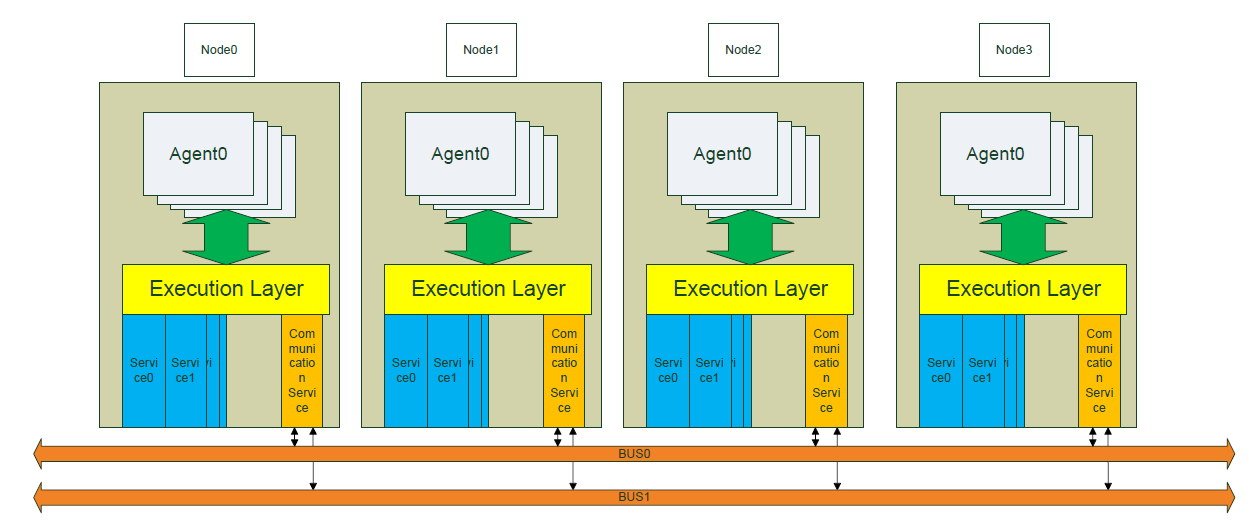
\includegraphics[scale=0.4]{figures/global.png}
\caption{Overview}
\end{figure}

On each of the 4 nodes, which can be found on the ESE board, a virtualization platform will be deployed. 
This virtualization platform will be able to execute up to 4 agents concurrently. The agents will be 
programmed in a simplistic assembler like agent language. On the platform there will be an execution 
layer which is able to execute the agent language. The agents will be able to access the hardware attached
to a node via services which are provided by the virtualization platform. Additionally the agents can
reproduce themselves to another node or even board. Within the platform a scheduler will be responsible for
providing execution time to each of the agents according to their priority. 

\section{Virtualization Platform}
The main task of the virtualization platform is to interprete the agent language commands of the agents 
and to provide them access to the hardware attached to a node via well defined interfaces. Additionally 
the platform should allow the concurrent execution of the agents. Therefore some basic means for code and 
data protection for the agent memory is required. This is achieved by assigning each of the agents an own 
memory segment and not allowing any other agent to access any other memory but its own. If some collaboration 
between the agents is required this must be requested via the communication service. The metadata of an agent 
as its code and memory segment will be stored in a structure that is shown in the figure below. 


\begin{figure}[!htb]
\lstset{language=C}
\begin{lstlisting}[frame=single]
typedef struct {

	uint8_t id;	
	uint8_t priority;
	agent_status_t status;

	uint32_t status_flag;
	uint16_t pc;

	int16_t regs[REG_MAX];

	uint16_t code_len;
	uint16_t regstr_len [STR_REG_MAX];

	uint16_t* code;

	char** reg_str;

	volatile char* rec_msg_content;
	volatile uint16_t rec_msg_len;
	
} agent_t;
\end{lstlisting}
\caption{Agent structure}
\label{agent}
\end{figure}

Every agent has a unique id within the virtualization platform. Additionally a priority and a status for the
scheduler are stored. Assigning these values for an agent lies within the scope of an agent developer. 
Reproducing an agent on a virtualization platform where the agent’s id is already used will result in a denial 
of the reproduction by the platform. Every agent has 13 numerical general purpose registers used for the execution
of the agent language. Additonally there are 3 char general purpose registers. The result of every agent language 
command will be written to the accumulator. There is also a program counter which is used for the execution of the
agent and the numerical agent language representation is stored as well. The agent structure also contains a buffer
for receiving messages from other agents.


\noindent
In order to reproduce the agent on another board or node the agent’s structure needs to be serialized and transmitted via the communication layer.


\noindent
Additionally the virtualization platform has to provide the agent developer with some means to deploy the agent
executable to the virtualization platform, during compilation of the platform. During the initialization of the
platform all deployed agents should be instantiated on the given platform.

\section{Execution Layer}

The execution layer is responsible for the execution of an agent which is written in the agent language and later translated to agent opcodes. 
The agent language provides means for:
\begin{itemize}
 \item storing values to the general purpose registers
 \item comparing the contents of the general purpose registers 
 \item performing basic mathematical functions like addition, subtraction, multiplication and division
 \item a jump operation 
 \item reproduction and cloning functions
 \item sleep, delay and terminate functions
 \item functions to access the hardware attached to a node
\end{itemize}


\noindent
If a function of the agent language returns a value, this value will be stored in the accumulator, 
where it can be used later on for further operations e.g. comparison etc. 


\noindent
The basic workflow of the execution layer as soon it is called by the scheduler is to read the next 
agent language opcode (all agent opcodes have a fixed length) as identified by the program counter, 
to decode it and to perform the function which is described by the opcode. Eventually the program 
counter value is changed and the control is returned back to the scheduler. 

\begin{figure}[!htbp]
\begin{center}
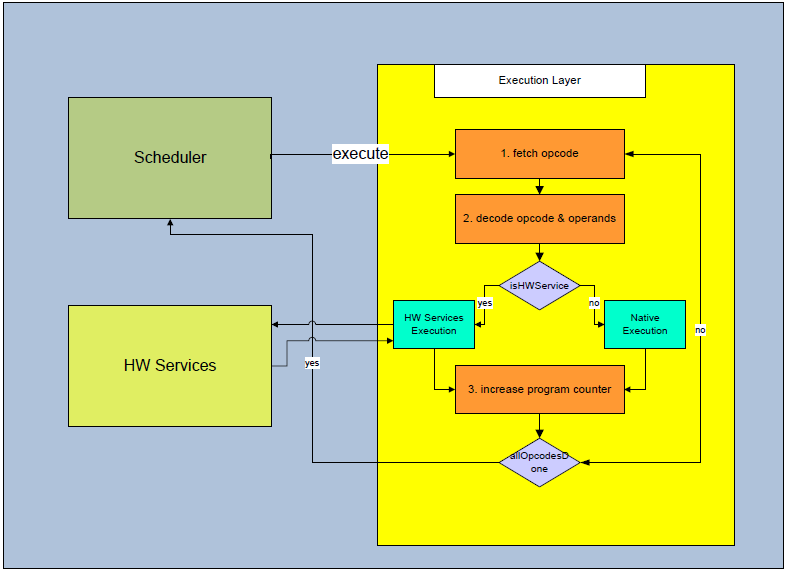
\includegraphics[scale=0.4]{figures/exelayer.png}
\caption{Execution Layer}
\end{center}
\label{exelayer}
\end{figure}



The execution layer is 
called by the method execute which takes the following input parameters:
\begin{itemize}
 \item Pointer to a specific agent structure
 \item Number of opcodes to execute
\end{itemize}

\begin{figure}[!htb]
\lstset{language=C}
\begin{lstlisting}[frame=single]
/**
	Function : execute_agent
		excutes the next opcodes of an agent
	Returns : 
		the amount of successfully executed opcoded
	Parameters : 
		agent : agent status structure
		opcode: amount of opcodes to be executed
**/
uint8_t execute_agent(agent_t *agent, uint8_t opcode_size);
\end{lstlisting}
\caption{Executing agent language opcode}
\label{fig:excopc}
\end{figure}



\section{Hardware Services}

The virtualization platform provides access to the hardware attached to a node via according hardware 
device drivers. The methods of the device drivers are made public to the execution layer which in turns 
allows the agents to access these methods. As the hardware supported by a node differs from node to node 
the virtualization platform should be able to discover during its initialization which hardware is supported 
on the node where it’s running. 


\noindent
This will be achieved by defining a global set of function pointers within the virtualization platform. 
This set should contain all possible methods of all available device drivers. During initialization the platform 
will assign the according function pointer to a method provided by the device driver if the device is supported, 
otherwise the according function pointer will stay null. 

\begin{figure}[!htb]
\lstset{language=C}
\begin{lstlisting}[frame=single]
typedef struct {

	void (*set_bargraph)(uint8_t value);

	uint32_t (*clk_get_time)(void);

	void (*set_cooler)(uint8_t duty_cycle);

	void (*DISPLAY_drawBg)(uint16_t rgb);

	void (*DISPLAY_drawDot)(uint8_t row, uint8_t col,
				uint16_t rgb, uint8_t grid);

	void (*DISPLAY_draw_char)(uint8_t x, uint8_t y, 
				uint16_t font_color, uint16_t bg_color, 
				uint8_t pixel_size, char c);
				
	void (*heater_set)(uint8_t duty_cycle);

	void(*button0_callback)(void);
	void(*button1_callback)(void);

	uint16_t (*therm_get_temp)(uint8_t name);

	void (*dotmatrix_send)(char *data);

} drivers_t;
\end{lstlisting}
\caption{Device drivers methods}
\label{fig:devicedrivers}
\end{figure}

\noindent
The platform detects all the supported drivers on a specific node by inspection of the linked drivers.
All drivers linked will be initialized during the setup of a platform and the methods provided by the 
drivers will be stored in the global function pointer table.
Choosing this approach we would reach some form of modularity which would allow us to exchange 
the device drivers without necessity to change the platform code.

\noindent
If an interaction with a device driver is blocking, then the calling agent will be put to status blocking unless there is an answer from
the device driver.

\section{Communication Layer}

The agents should be able to communicate with other agents on the same node or on the same board. Therefore the agent 
language provides means to request the sending or receiving of a message.  


\noindent
The sending function is blocking the further execution of the agent until the message is sent. 
When an agent wants to send a message this message is proceeded to the communications service which takes care of the 
actual transmission. While the sending procedure is ongoing the further execution of the sending agent is blocked.
As soon as the communication service signalizes a successful message transmission or a failure the result of the 
sending function is written to the accumulator and the agent will be made available for further execution.  


\noindent
When an agent sends a message to another agent, the receiving platform stores the content 
to the receiver agent structure. The receiving agent is able to retrieve the last message from its buffer. 
However only one message can be stored within the receiving agent structure and the next message will overwrite the 
content and possible the id of the last message.  


\noindent
The communication service provides no guarantees that sending of a message will succeed; it works on a best effort 
approach. Therefore the agent developer has to make sure by reading the return value of a sending operation whether 
the message was successfully sent or not and should initialize a retransmission in case of failure. 


\noindent
Every message sent should be identified by an id, in order to allow the transmission of messages with different semantics.

\noindent
The receiver of a message should be identified via the node number (0..3) where the receiving agent is currently expected
to be running and the receiver agent id. As the ids of agents are within the scope of the agent developer she has to make 
sure, that the correct receiving agent is addressed. Additionally a multicast message could be supported by allowing omitting 
the node address which should result in sending the message to all agents identified by the provided id. 

\section{Scheduler}
The main task of the scheduler which is part of the virtualization platform is to identify the next agent to be executed 
and to utilize the execution layer to perform the execution of the according agent. The decision which agent to be chosen 
should be made on a static priority based scheduling policy.


\noindent
Every agent is assigned a priority (0..254) by the agent developer which is stored within the agent structure. 
The highest priority is 254 and the lowest priority is 0. Based on the priorities of the currently running agents 
the scheduler creates a static list by which the order of the agent execution is defined. The scheduler instructs 
the execution layer to execute exactly priority + 1 opcodes for a given agent. Eventually the control returns to 
the scheduler and the next agent from the list is picked. The list is iterated cyclically.

\begin{figure}[!htbp]
\begin{center}
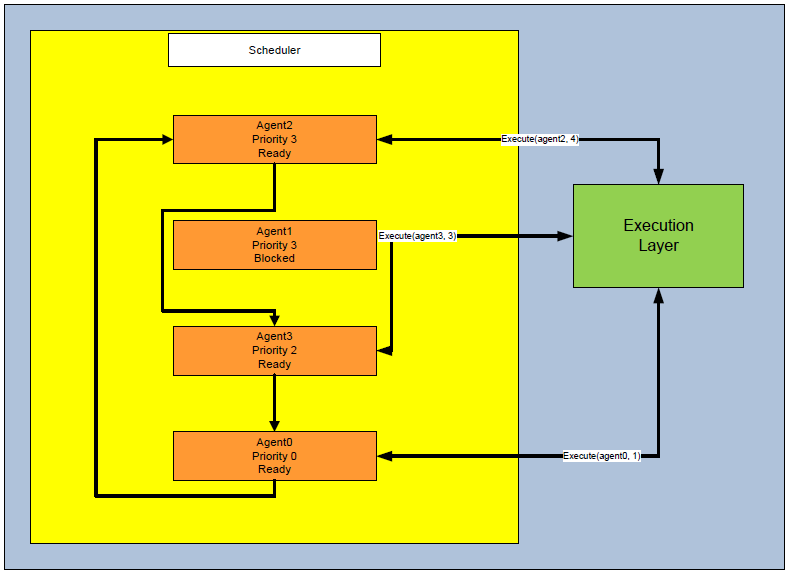
\includegraphics[scale=0.4]{figures/scheduler.png}
\caption{Scheduler}
\end{center}
\label{scheduler}
\end{figure}


\noindent
If an agent which is to be scheduled next is currently blocked, then its execution should be omitted. 


\noindent
As an agent can reproduce it self to another node or board or clone itself within the same platform the scheduling 
list requires adaptation as soon as new agent is deployed on a platform. Whenever a given platform is the destination 
end point of a reproduction respectively cloning operation the scheduler needs to update its scheduling list before proceeding with further executions.

\section{Agent language}

\subsection{Agent language (Assembler level)}
\noindent
To develop a mobile agent \textit{Agent language} will be used. Language is tied to agent internal structure and support necessary operation for code mobility and message exchange. While writing the program for agent user should not be aware of hardware services presented on a given platform, but have common knowledge about all available services and what operations are allowed to do with the services (have list of services and available operations). It is the responsibility of the platform to provide required service to the agent (perform measurement, IO operation) or to manifest an error if the service is not available on the given platform. All current variables are allowed to store only in registers of agent structure (Fig. ~\ref{agent}).


\noindent
The language supports the following groups of operations: arithmetic, control flow, code mobility, message exchange , access to hardware services.


\begin{tabular}{|l|c|l|c|}
\hline
\multicolumn{4}{|c|}{\textbf{Addressing registers of agent structure}}\\
\hline
\multicolumn{2}{|c|}{\textbf{General purpose registers}} & \multicolumn{2}{c|}{\textbf{Character registers}}\\
\hline
Register & \texttt{rrrr} & Char Register & \texttt{rrrr}\\
\hline
\texttt{reg_0} & \texttt{0000} & \texttt{reg_str_0} & \texttt{1101}\\
\hline
\texttt{reg_1} & \texttt{0001} & \texttt{reg_str_1} & \texttt{1110}\\
\hline
\texttt{reg_2} & \texttt{0010} & \texttt{reg_str_2} & \texttt{1111}\\
\hline
\texttt{reg_3} & \texttt{0011} &   &  \\
\hline
\texttt{reg_4} & \texttt{0100} &   &  \\
\hline
\texttt{reg_5} & \texttt{0101} &   &  \\
\hline
\texttt{reg_6} & \texttt{0110} &   &  \\
\hline
\texttt{reg_7} & \texttt{0111} &   &  \\
\hline
\texttt{reg_8} & \texttt{1000} &   &  \\
\hline
\texttt{reg_9} & \texttt{1001} &   &  \\
\hline
\texttt{reg_10} & \texttt{1010} &   &  \\
\hline
\texttt{reg_11} & \texttt{1011} &   &  \\
\hline
\texttt{reg_12} & \texttt{1100} &   &  \\
\hline
%\texttt{acc} & \texttt{1111} & &\\
%\hline
%\texttt{reg_7L} & \texttt{0111} &   &  \\
%\hline
%\texttt{reg_7H} & \texttt{1011} &  &  \\
%\hline
%\texttt{reg_7} & \texttt{1100} & & \\

%\hline
\end{tabular}

\subsubsection{Arithmetic operations of agent assembly language}
\noindent
\textbf{Addition}

\noindent
Add the content of \texttt{reg_d} and \texttt{reg_r} (or \texttt{value}) and put the result into \texttt{reg_0}.\\
\noindent
\framebox{\texttt{add reg_d, reg_r}}

\noindent
\begin{tabular}{+p{1.3in}+p{2.2in}+p{1.3in}+p{1in}}

Syntax  & Operands   & Program counter & Flags\\

\texttt{add reg_d, reg_r} & \texttt{reg_0 $\leq$ reg_d $\leq$ reg_12,  reg_0 $\leq$ reg_r $\leq$ reg_12} & \texttt{PC = PC + 1} & \texttt{C} \\

\multicolumn{2}{l}{Operation} & & \\

\multicolumn{2}{l}{\texttt{reg_0 $\leftarrow$ reg_d + reg_r}} & & \\

\end{tabular}

\noindent
16-bit opcode:

\noindent
\begin{tabular}{|c|c|c|c|}
\multicolumn{2}{|l|}{} & reg_d & reg_r\\
\hline
\texttt{0000} & \texttt{0011} & \texttt{dddd} & \texttt{rrrr}\\

\end{tabular}

\vspace{0.5in}
\noindent
\framebox{\texttt{add reg_r, value}}
\vspace{0.2in}

\noindent
\begin{tabular}{+p{1.3in}+p{2.2in}+p{1.3in}+p{1in}}

Syntax  & Operands   & Program counter & Flags\\

\texttt{add reg_r, value} & \texttt{reg_0 $\leq$ reg_r $\leq$ reg_12, 0x00 $\leq$ value $\leq$ 0xFF} & \texttt{PC = PC + 1} & \texttt{C} \\

\multicolumn{2}{l}{Operation} & & \\

\multicolumn{2}{l}{\texttt{reg_0 $\leftarrow$ reg_r + value}} & & \\

\end{tabular}

\noindent
16-bit opcode:

\noindent
\begin{tabular}{|c|c|c|c|}
 & reg_r & \multicolumn{2}{c|}{value}\\
\hline
\texttt{0011} & \texttt{rrrr} & \texttt{vvvv} & \texttt{vvvv}\\

\end{tabular}

\vspace{0.5in}

\noindent
\textbf{Subtraction}

\noindent
Subtract \texttt{reg_s} (or \texttt{value}) from \texttt{reg_m} and put the result into \texttt{reg_0}.\\
\noindent
\framebox{\texttt{sub reg_m, reg_s}}

\noindent
\begin{tabular}{+p{1.3in}+p{2.2in}+p{1.3in}+p{1in}}

Syntax  & Operands   & Program counter & Flags\\

\texttt{sub reg_m, reg_s} & \texttt{reg_0 $\leq$ reg_m $\leq$ reg_12, reg_0 $\leq$ reg_s $\leq$ reg_12,} & \texttt{PC = PC + 1} & \texttt{C} \\

\multicolumn{2}{l}{Operation} & & \\

\multicolumn{2}{l}{\texttt{reg_0 $\leftarrow$ reg_m - reg_s}} & & \\

\end{tabular}

\noindent
16-bit opcode:

\noindent
\begin{tabular}{|c|c|c|c|}
\multicolumn{2}{|l|}{} & reg_m & reg_s\\
\hline
\texttt{0000} & \texttt{0110} & \texttt{mmmm} & \texttt{ssss}\\

\end{tabular}

\vspace{0.5in}
\noindent
\framebox{\texttt{sub reg_m, value}}
\vspace{0.1in}

\noindent
\begin{tabular}{+p{1.3in}+p{2.2in}+p{1.3in}+p{1in}}

Syntax  & Operands   & Program counter & Flags\\

\texttt{sub reg_m, value} & \texttt{reg_0 $\leq$ reg_m $\leq$ reg_12, 0x00 $\leq$ value $\leq$ 0xFF} & \texttt{PC = PC + 1} & \texttt{C} \\

\multicolumn{2}{l}{Operation} & & \\

\multicolumn{2}{l}{\texttt{reg_0 $\leftarrow$ reg_m - value}} & & \\

\end{tabular}

\noindent
16-bit opcode:

\noindent
\begin{tabular}{|c|c|c|c|}
 & reg_m & \multicolumn{2}{c|}{value}\\
\hline
\texttt{0110} & \texttt{mmmm} & \texttt{vvvv} & \texttt{vvvv}\\

\end{tabular}

\vspace{0.5in}



\noindent
\textbf{Division}

\noindent
Divide \texttt{reg1} by \texttt{reg2} (or value) and put the result into \texttt{reg_0}.\\
\noindent
\framebox{\texttt{div reg_d, reg_r}}

\noindent
\begin{tabular}{+p{1.3in}+p{2.2in}+p{1.3in}+p{1in}}

Syntax  & Operands   & Program counter & Flags\\

\texttt{div reg_d, reg_r} & \texttt{reg_0 $\leq$ reg_d $\leq$ reg_12, reg_0 $\leq$ reg_r $\leq$ reg_12,} & \texttt{PC = PC + 1} & \texttt{C} \\

\multicolumn{2}{l}{Operation} & & \\

\multicolumn{2}{l}{\texttt{reg_0 $\leftarrow$ reg_d / reg_r}} & & \\

\end{tabular}

\noindent
16-bit opcode:

\noindent
\begin{tabular}{|c|c|c|c|}
\multicolumn{2}{|l|}{} & reg_d & reg_r\\
\hline
\texttt{0000} & \texttt{1001} & \texttt{dddd} & \texttt{rrrr}\\

\end{tabular}

\vspace{0.5in}
\noindent
\framebox{\texttt{div reg_d, value}}
\vspace{0.1in}

\noindent
\begin{tabular}{+p{1.3in}+p{2.2in}+p{1.3in}+p{1in}}

Syntax  		  & Operands   								     & Program counter       & Flags\\

\texttt{div reg_d, value} & \texttt{reg_0 $\leq$ reg_d $\leq$ reg_12,  0x00 $\leq$ value $\leq$ 0xFF} & \texttt{PC = PC + 1} & \texttt{C} \\

\multicolumn{2}{l}{Operation} 									      & 		     & \\

\multicolumn{2}{l}{\texttt{reg_0 $\leftarrow$ reg_d / value}} & & \\

\end{tabular}

\noindent
16-bit opcode:

\noindent
\begin{tabular}{|c|c|c|c|}
 & reg_d & \multicolumn{2}{c|}{value}\\
\hline
\texttt{1001} & \texttt{dddd} & \texttt{vvvv} & \texttt{vvvv}\\

\end{tabular}

\vspace{0.2in}

\noindent
\textbf{Multiplication}


\noindent
Multiply \texttt{reg1} and \texttt{reg2} (or \texttt{value}) and put the result into \texttt{reg_0}.\\
\noindent
\framebox{\texttt{mul reg_d, reg_r}}

\noindent
\begin{tabular}{+p{1.3in}+p{2.2in}+p{1.3in}+p{1in}}

Syntax  & Operands   & Program counter & Flags\\

\texttt{mul reg_d, reg_r} & \texttt{reg_0 $\leq$ reg_d $\leq$ reg_12, reg_0 $\leq$ reg_r $\leq$ reg_12 } & \texttt{PC = PC + 1} & \texttt{C} \\

\multicolumn{2}{l}{Operation} & & \\

\multicolumn{2}{l}{\texttt{reg_0 $\leftarrow$ reg_d * reg_r}} & & \\

\end{tabular}

\noindent
16-bit opcode:

\noindent
\begin{tabular}{|c|c|c|c|}
\multicolumn{2}{|l|}{} & reg_d & reg_r\\
\hline
\texttt{0000} & \texttt{1100} & \texttt{dddd} & \texttt{rrrr}\\

\end{tabular}

\vspace{0.5in}
\noindent
\framebox{\texttt{mul reg1, value}}
\vspace{0.1in}

\noindent
\begin{tabular}{+p{1.3in}+p{2.2in}+p{1.3in}+p{1in}}

Syntax  		  & Operands   								     & Program counter       & Flags\\

\texttt{mul reg_d, value} & \texttt{reg_0 $\leq$ reg_d $\leq$ reg_12, 0x00 $\leq$ value $\leq$ 0xFF} & \texttt{PC = PC + 1} & \texttt{C} \\

\multicolumn{2}{l}{Operation} 									      & 		     & \\

\multicolumn{2}{l}{\texttt{reg_0 $\leftarrow$ reg_d * value}} & & \\

\end{tabular}

\noindent
16-bit opcode:

\noindent
\begin{tabular}{|c|c|c|c|}
 & reg_d & \multicolumn{2}{c|}{value}\\
\hline
\texttt{1100} & \texttt{dddd} & \texttt{vvvv} & \texttt{vvvv}\\

\end{tabular}


\subsubsection{Control flow operations and comparison in agent assembly language}
\noindent
\textbf{Jump if greater}

\noindent
Jump to  \texttt{offset} in code segment of agent structure if the value of \texttt{reg_0}. is 1.

\noindent
\framebox{\texttt{jmpgr  offset}}
\vspace{0.1in}

\noindent
\begin{tabular}{+p{1.3in}+p{2.1in}+p{2.5in}}
Syntax  		  & Operands   								     & Program counter       \\

\texttt{jmpgr  offset} & \texttt{-128 $\leq$ offset $\leq$ +127} & \texttt{PC = PC + offset +1} if \texttt{reg_0 = 1}, \texttt{PC = PC + 1} otherwise \\

\end{tabular}

\noindent
16-bit opcode:

\noindent
\begin{tabular}{|c|c|c|c|}
 \multicolumn{2}{|c|}{} & \multicolumn{2}{c|}{offset}\\
\hline
\texttt{1111} & \texttt{0011} & \texttt{vvvv} & \texttt{vvvv}\\

\end{tabular}

\vspace{0.4in}
\noindent
\textbf{Jump if equal}

\noindent
Jump to \texttt{offset} in code segment of agent structure if the value of \texttt{reg_0} is 0.

\noindent
\framebox{\texttt{jmpeq  offset}}
\vspace{0.1in}

\noindent
\begin{tabular}{+p{1.3in}+p{2.1in}+p{2.5in}}
Syntax  		  & Operands   								     & Program counter       \\

\texttt{jmpeq  offset} & \texttt{-128 $\leq$ offset $\leq$ +127} & \texttt{PC = PC + offset +1} if \texttt{reg_0 = 0}, \texttt{PC = PC + 1} otherwise \\

\end{tabular}

\noindent
16-bit opcode:

\noindent
\begin{tabular}{|c|c|c|c|}
 \multicolumn{2}{|c|}{} & \multicolumn{2}{c|}{offset}\\
\hline
\texttt{1111} & \texttt{0110} & \texttt{vvvv} & \texttt{vvvv}\\

\end{tabular}


\vspace{0.4in}
\noindent
\textbf{Jump if less}

\noindent
Jump to \texttt{offset} in code segment of agent structure if the value of \texttt{reg_0} is -1.

\noindent
\framebox{\texttt{jmpls  offset}}

\vspace{0.1in}

\noindent
\begin{tabular}{+p{1.3in}+p{2.1in}+p{2.7in}}
Syntax  		  & Operands   								     & Program counter       \\

\texttt{jmpls  offset} & \texttt{-128 $\leq$ offset $\leq$ +127} & \texttt{PC = PC + offset +1} if \texttt{reg_0 = -1}, \texttt{PC = PC + 1} otherwise \\

\end{tabular}

\noindent
16-bit opcode:

\noindent
\begin{tabular}{|c|c|c|c|}
 \multicolumn{2}{|c|}{} & \multicolumn{2}{c|}{offset}\\
\hline
\texttt{1111} & \texttt{1100} & \texttt{vvvv} & \texttt{vvvv}\\

\end{tabular}

\vspace{0.4in}
\noindent
\textbf{Comparison}

\noindent
Compare \texttt{reg1} and \texttt{reg2} (or \texttt{value}).

%\noindent
%If reg1 $>$ reg2 put 1 into acc,

%\noindent
%if reg1 $=$ reg2 put 0 into acc,

%\noindent
%if reg1 $<$ reg2 put -1 into acc.

\noindent
\framebox{\texttt{compare reg_d, reg_r}}

\noindent
\begin{tabular}{+p{1.8in}+p{2.2in}+p{1.3in}}

Syntax  & Operands   & Program counter \\

\texttt{compare reg_d, reg_r} & \texttt{reg_0 $\leq$ reg_d $\leq$ reg_12, reg_0 $\leq$ reg_r $\leq$ reg_12 } & \texttt{PC = PC + 1} \\

\multicolumn{3}{l}{Operation} \\

\multicolumn{2}{l}{\texttt{reg_0 $\leftarrow$ 1} if (reg_d - reg_r $>$ 0)}  & \\
\multicolumn{2}{l}{\texttt{reg_0 $\leftarrow$ 0} if (reg_d - reg_r $=$ 0)}  & \\
\multicolumn{2}{l}{\texttt{reg_0 $\leftarrow$ -1} if (reg_d - reg_r $<$ 0)}  & \\
\end{tabular}

\noindent
16-bit opcode:

\noindent
\begin{tabular}{|c|c|c|c|}
\multicolumn{2}{|l|}{} & reg_d & reg_r\\
\hline
\texttt{0000} & \texttt{1010} & \texttt{dddd} & \texttt{rrrr}\\

\end{tabular}

\vspace{0.4in}
\noindent
\framebox{\texttt{compare reg_d, value}}

\noindent
\begin{tabular}{+p{1.9in}+p{2.2in}+p{1.3in}}

Syntax  & Operands   & Program counter \\

\texttt{compare reg_d, value} & \texttt{reg_0 $\leq$ reg_d $\leq$ reg_12, 0x00 $\leq$ value $\leq$ 0xFF} & \texttt{PC = PC + 1} \\

\multicolumn{3}{l}{Operation} \\

\multicolumn{2}{l}{\texttt{reg_0 $\leftarrow$ 1} if (reg_d - value $>$ 0)}  & \\
\multicolumn{2}{l}{\texttt{reg_0 $\leftarrow$ 0} if (reg_d - value $=$ 0)}  & \\
\multicolumn{2}{l}{\texttt{reg_0 $\leftarrow$ -1} if (reg_d - value $<$ 0)}  & \\
\end{tabular}

\noindent
16-bit opcode:

\noindent
\begin{tabular}{|c|c|c|c|}
 & reg_r & \multicolumn{2}{c|}{value}\\
\hline
\texttt{1010} & \texttt{rrrr} & \texttt{vvvv} & \texttt{vvvv}\\

\end{tabular}

\vspace{0.5in}

\subsubsection{Code mobility operations of agent assembly language}
\noindent
\textbf{Move code}

\noindent
Move agent structure to platform that possess required service

\noindent
\framebox{\texttt{move service}}
\vspace{0.1in}

\begin{tabular}{+p{1.3in}+p{2.8in}+p{1.3in}}

Syntax  & Operands   & Program counter \\

\texttt{move service} & \texttt{service_0 $\leq$ service $\leq$ service_255} & \texttt{PC = PC + 1} \\

\multicolumn{3}{l}{Operation} \\

\multicolumn{3}{l}{Serialize and transmit agent structure to the platform that possess required service}  \\

\end{tabular}

\vspace{0.1in}
\noindent
16-bit opcode:

\noindent
\begin{tabular}{|c|c|c|c|}
 & reg_r & \multicolumn{2}{c|}{service}\\
\hline
\texttt{1111} & \texttt{0001} & \texttt{ssss} & \texttt{ssss}\\

\end{tabular}

\vspace{0.5in}
\noindent
\textbf{Clone code}

\noindent
Replicate agent structure on the given platform

\noindent
\framebox{\texttt{clone}}
\vspace{0.1in}

\begin{tabular}{+p{1.3in}+p{1.3in}}

Syntax    & Program counter \\

\texttt{clone}  & \texttt{PC = PC + 1} \\

\end{tabular}

\vspace{0.1in}
\noindent
16-bit opcode:

\noindent
\begin{tabular}{|c|c|c|c|}
  \multicolumn{4}{|c|}{}\\
\hline
\texttt{1111} & \texttt{0010} & \texttt{0000} & \texttt{0000}\\

\end{tabular}

\vspace{0.4in}
\noindent
\textbf{Die}

\noindent
Destroy agent structure and free corresponding memory

\noindent
\framebox{\texttt{die}}

\vspace{0.1in}
\noindent
16-bit opcode:

\noindent
\begin{tabular}{|c|c|c|c|}
  \multicolumn{4}{|c|}{}\\
\hline
\texttt{1111} & \texttt{0100} & \texttt{0000} & \texttt{0000}\\
\end{tabular}

\subsubsection{Message exchange}
\noindent
\textbf{Send}
Message exchange between agents
\noindent


\noindent
\framebox{\texttt{sendmsg reg, agent, platform}}
\vspace{0.1in}


\noindent
\begin{tabular}{+p{2.3in}+p{3.0in}+p{1.2in}}

Syntax  & Operands   & Program counter \\

\texttt{sendmsg reg, agent, platform} & \texttt{platform_0 $\leq$ platform $\leq$ platform_3} & \texttt{PC = PC + 1}\\
 & \texttt{agent_0 $\leq$ agent $\leq$ agent_3} & \\
 & \texttt{reg_0 $\leq$ reg $\leq$ reg_12} & \\
 & \texttt{reg_str_0 $\leq$ reg $\leq$ reg_str_2} & \\
\multicolumn{3}{l}{Operation} \\
\multicolumn{3}{l}{Send value of the register \texttt{reg} to the agent \texttt{aa} on the platform \texttt{pp}} \\

\end{tabular}

\noindent
16-bit opcode:

\noindent
\begin{tabular}{|c|c|c|c|c|}
 \multicolumn{2}{|c|}{} & register & agent & platform\\
\hline
\texttt{1111} & \texttt{1000} & \texttt{rrrr} &\texttt{aa} & \texttt{pp}\\

\end{tabular}


\vspace{0.5in}
\noindent
\textbf{Receive}

\noindent
Pull message from \texttt{platform} to \texttt{register}.

\noindent
\framebox{\texttt{pullmsg reg}}

\noindent
\begin{tabular}{+p{1.9in}+p{3.0in}+p{1.3in}}

Syntax & Operation  & Program counter \\

\texttt{pullmsg} & \texttt{reg_0 $\leq$ reg $\leq$ reg_12} & \texttt{PC = PC + 1} \\
 & \texttt{reg_str_0 $\leq$ reg $\leq$ reg_str_2} & \\

\multicolumn{3}{l}{Operation} \\

\multicolumn{3}{l}{ \texttt{reg $\leftarrow$} message} \\

\end{tabular}

\noindent
16-bit opcode:

\noindent
\begin{tabular}{|c|c|c|c|}
 \multicolumn{2}{|c|}{} & & \texttt{rrrr} \\
\hline
\texttt{1111} & \texttt{1010} & \texttt{0000} & \texttt{0000}\\
\end{tabular}

\vspace{0.1in}
\subsubsection{Store, move and wait operations}
\noindent
\textbf{Store}


\noindent
Store \texttt{value} in \texttt{h}-part of \texttt{reg_d}

\noindent
\framebox{\texttt{ldh reg_d, value}}

\noindent
\begin{tabular}{+p{1.8in}+p{2.2in}+p{1.3in}}

Syntax  		  & Operands   								     & Program counter       \\

\texttt{ldh reg_d, value} & \texttt{reg_0 $\leq$ reg_d $\leq$ reg_12, 0x00 $\leq$ value $\leq$ 0xFF} & \texttt{PC = PC + 1}  \\

\multicolumn{2}{l}{Operation} 									      & 		     \\

\multicolumn{2}{l}{\texttt{reg_d_h $\leftarrow$ value}} & \\

\end{tabular}

\noindent
16-bit opcode:

\noindent
\begin{tabular}{|c|c|c|c|}
 & reg_d & \multicolumn{2}{c|}{value}\\
\hline
\texttt{1101} & \texttt{dddd} & \texttt{vvvv} & \texttt{vvvv}\\

\end{tabular}

\vspace{0.4in}
\noindent
Store \texttt{value} in \texttt{l}-part of \texttt{reg_d}

\noindent
\framebox{\texttt{ldl reg_d, value}}

\noindent
\begin{tabular}{+p{1.8in}+p{2.2in}+p{1.3in}}

Syntax  		  & Operands   								     & Program counter       \\

\texttt{ldl reg_d, value} & \texttt{reg_0 $\leq$ reg_d $\leq$ reg_12, 0x00 $\leq$ value $\leq$ 0xFF} & \texttt{PC = PC + 1}  \\

\multicolumn{2}{l}{Operation} 									      & 		     \\

\multicolumn{2}{l}{\texttt{reg_d_l $\leftarrow$ value}} & \\

\end{tabular}

\noindent
16-bit opcode:

\noindent
\begin{tabular}{|c|c|c|c|}
 & reg_d & \multicolumn{2}{c|}{value}\\
\hline
\texttt{0100} & \texttt{dddd} & \texttt{vvvv} & \texttt{vvvv}\\
\end{tabular}
\vspace{0.4in}

\noindent
Push \texttt{char} value in the \texttt{str_reg}
\vspace{0.1in}
\noindent

\framebox{\texttt{storecr reg_str, char}}
\vspace{0.1in}

\noindent
\begin{tabular}{+p{1.8in}+p{2.9in}+p{1.3in}}

Syntax  		  & Operands   						    & Program counter       \\

\texttt{storecr reg_str, char} & \texttt{reg_str_0 $\leq$ reg_str $\leq$ reg_str_2} & \texttt{PC = PC + 1}  \\

\multicolumn{2}{l}{Operation} 									      & 		     \\

\multicolumn{2}{l}{\texttt{reg_str $\Leftarrow$ value}} & \\

\end{tabular}

\noindent
16-bit opcode:

\noindent
\begin{tabular}{|c|c|c|c|}
 & reg_str & \multicolumn{2}{c|}{value}\\
\hline
\texttt{1011} & \texttt{rrrr} & \texttt{vvvv} & \texttt{vvvv}\\

\end{tabular}

\vspace{0.4in}

\noindent
Clear the \texttt{str_reg}
\vspace{0.1in}
\noindent

\framebox{\texttt{clr reg_str}}
\vspace{0.1in}

\noindent
\begin{tabular}{+p{1.8in}+p{2.9in}+p{1.3in}}

Syntax  		  & Operands   						    & Program counter       \\

\texttt{clr str_reg} & \texttt{reg_str_0 $\leq$ reg_str $\leq$ reg_str_2} & \texttt{PC = PC + 1}  \\

\multicolumn{2}{l}{Operation} 									      & 		     \\

\multicolumn{2}{l}{\texttt{clear str_reg}} & \\

\end{tabular}

\noindent
16-bit opcode:

\noindent
\begin{tabular}{|c|c|c|c|}
\multicolumn{3}{|c|}{} & {rrrr}\\
\hline
\texttt{0000} & \texttt{0010} & \texttt{0000} & \texttt{rrrr}\\

\end{tabular}

\vspace{0.4in}

\noindent
\textbf{Move}

\noindent
Move value from reg_r to reg_d

\noindent
\framebox{\texttt{mv reg_d, reg_r}}

\noindent
\begin{tabular}{+p{1.8in}+p{2.2in}+p{1.3in}}

Syntax  		  & Operands   								     & Program counter       \\

\texttt{mv reg_d, reg_r} & \texttt{reg_0 $\leq$ reg_d $\leq$ reg_12,  reg_0 $\leq$ reg_r $\leq$ reg_12} & \texttt{PC = PC + 1}  \\

\multicolumn{2}{l}{Operation} 									      & 		     \\

\multicolumn{2}{l}{\texttt{reg_d $\leftarrow$ reg_r}} & \\

\end{tabular}

\noindent
16-bit opcode:

\noindent
\begin{tabular}{|c|c|c|c|}
 \multicolumn{2}{|c|}{} & reg_d & reg_r\\
\hline
\texttt{0000} & \texttt{1101} & \texttt{dddd} & \texttt{rrrr}\\

\end{tabular}

\vspace{0.5in}

\noindent
\textbf{Wait}

\noindent
Wait for ms


\noindent
\framebox{\texttt{wait delay_ms}}

\noindent
\begin{tabular}{+p{1.8in}+p{2.2in}+p{1.3in}}

Syntax  		  & Operands   								     & Program counter       \\

\texttt{wait delay_ms} & \texttt{0 $\leq$ delay_ms $\leq$ 0xFF} & \texttt{PC = PC + 1}  \\


\end{tabular}

\noindent
16-bit opcode:

\noindent
\begin{tabular}{|c|c|c|c|}
 \multicolumn{2}{|c|}{} & \multicolumn{2}{c|}{delay}\\
\hline
\texttt{0000} & \texttt{0101} & \texttt{dddd} & \texttt{dddd}\\

\end{tabular}
\vspace{0.4in}

\noindent
\textbf{Assign priority value}


\noindent
Assign priority of the agent to value in range 0..3

\noindent
\framebox{\texttt{priority value}}


\noindent
\begin{tabular}{+p{1.8in}+p{2.2in}+p{1.3in}}

Syntax  		  & Operands   								     & Program counter       \\

\texttt{priority value} & \texttt{0 $\leq$ value $\leq$ 3} & \texttt{PC = PC + 1}  \\

\multicolumn{2}{l}{Operation} 									      & 		     \\

\multicolumn{2}{l}{\texttt{priority $\leftarrow$ value}} & \\

\end{tabular}

\noindent
16-bit opcode:

\noindent
\begin{tabular}{|c|c|c|c|}
 \multicolumn{2}{|c|}{} &  \multicolumn{2}{c|}{priority}\\
\hline
\texttt{0000} & \texttt{1000} & \texttt{pppp} & \texttt{pppp}\\

\end{tabular}

\vspace{0.4in}
\subsubsection{Access to hardware services}
\noindent
\textbf{Set}

\noindent
Set service to reg or value

\noindent
\framebox{\texttt{setservice service_id, reg}}

\noindent
\begin{tabular}{+p{1.9in}+p{3.1in}+p{1.2in}}

Syntax  		  & Operands   								     & Program counter       \\

\texttt{setservice service_id, reg} & \texttt{service_0 $\leq$ service_id $\leq$ service_255, reg_0 $\leq$ reg $\leq$ reg_12} & \texttt{PC = PC + 1}  \\

\end{tabular}

\noindent
16-bit opcode:

\noindent
\begin{tabular}{|c|c|c|c|}
 & reg & \multicolumn{2}{c|}{service_id}\\
\hline
\texttt{0111} & \texttt{rrrr} & \texttt{ssss} & \texttt{ssss}\\

\end{tabular}
\vspace{0.1in}
%\noindent
%\framebox{\texttt{setservice value}}
%\vspace{0.1in}

\noindent
\textbf{Get}

\noindent
Put corresponding value from the service to the \texttt{reg_0}.

\noindent
\framebox{\texttt{getservice service\_id}}
\vspace{0.1in}

\noindent
\begin{tabular}{+p{1.9in}+p{3.0in}+p{1.2in}}

Syntax  & Operand  & Program counter       \\

\texttt{getservice service_id}& service_0 $\leq$ service_id $\leq$ service_255 & \texttt{PC = PC + 1}  \\

\end{tabular}

\noindent
16-bit opcode:

\noindent
\begin{tabular}{|c|c|c|c|}
 \multicolumn{2}{|c|}{} &\multicolumn{2}{c|}{service_id} \\
\hline
\texttt{0000} & \texttt{0111} & \texttt{ssss} & \texttt{ssss}\\

\end{tabular}
\vspace{0.1in}

\begin{comment}
, comparison of operands, jump and loop constructs, as well as operations related to code mobility ( move to service, clone, die). Developer of agent program should not be aware of present services on the 
The agent developer use the following language to develop the program.
Program consist of single possible recursive function. The language has two types: integer and string.


\begin{longtable}{|l|p{5in}|}
\hline
Lexical elements	
&
Agent program includes the following lexical elements
\\
\hline
keyword
&
'function' $~\mid~$ 'var' $~\mid~$ 'int' $~\mid~$ 'char' $~\mid~$ 'boolean' $~\mid~$ 'true' $~\mid~$ 'false' $~\mid~$ 'this' $~\mid~$ 'if' $~\mid~$ 'else' $~\mid~$ 'while' $~\mid~$ 'return' $~\mid~$ 'move' $~\mid~$ 'clone' $~\mid~$  'message' $~\mid~$  'to'  $~\mid~$  
\\
\hline
symbol
&
$~\mid~$  '\{'  $~\mid~$  '\}'  $~\mid~$  '('  $~\mid~$  ')'  $~\mid~$  '['  $~\mid~$  ']'  $~\mid~$  '.'  $~\mid~$  ','  $~\mid~$  ';'  $~\mid~$  '+'  $~\mid~$  '-'  $~\mid~$  '*'  $~\mid~$  '/'  $~\mid~$  '\&'  $~\mid~$  '$~\mid~$'  $~\mid~$  '<'  $~\mid~$  '>'  $~\mid~$  '='  $~\mid~$  '\~ 	'	
\\
\hline
intConstant
&
a number in range $0 \ldots 2^{16}$
\\
\hline
stringConstant
&
' " ' a sequence of Unicode characters including in double quotes ' " '
\\
\hline
identifier
&
A sequence of letters, digits, and underscore('_') starting with a letter
\\
\hline
boardIdentifier
&
Board1 $~\mid~$ Board2
\\
\hline
platformIdentifier
&
boardIdentifier.(Platform1 $~\mid~$ Platform2 $~\mid~$ Platform3 $~\mid~$ Platform4)
\\
\hline
serviceIdentifier
&
boardIdenttifier.platformIdentifier.( serviceA $~\mid~$ serviceB $~\mid~$ serviceC $~\mid~$ serviceD $~\mid~$ serviceE $~\mid~$ serviceF1 $~\mid~$  serviceF2 $~\mid~$ serviceG )
\\
\hline
agentIdentifier
&
indentifier
\\
\hline
Program structure
&
Structure of Agent program
\\
\hline
function declaration
&
'function' ( 'void' $~\mid~$ type) functionName '(' parameterList ')' functionBody
\\
\hline
parameterList
&
((type varName) (',' type varName)*)?
\\
\hline
functionBody
&
'{' varDec* statements  '}'
\\
\hline
varDec
&
'var' type varName (',' varName)* ';'
\\
\hline
functionName
&
identifier
\\
\hline
varName
&
identifier
\\
\hline
Statements
&
Statements in Agent program
\\
\hline
statements
&
statement*
\\
\hline
statement
&
decStatement $~\mid~$ ifStatement $~\mid~$ whileStatement $~\mid~$ returnStatement $~\mid~$ dieStatement
\\
\hline
decStatement
&
varName ( '[' expression ']' )? '=' expression ';'
\\
\hline
ifStatement
&
if '(' expression ')' '{' statements '}' (else '{' statements '}')?
\\
\hline
whileStatement
&
while '(' expression ')'  '{'  statements '}'
\\
\hline
returnStatement
&
return expression? ';'
\\
\hline
moveStatement
&
move to (platformIdentifier  $~\mid~$ serviceIdentifier) ';'
\\
\hline
cloneStatement
&
clone ';'
\\
\hline
messageStatement
&
message '(' expression ')' to (platformIdentifier $~\mid~$ agentIdentifier ) ';'
\\
\hline
getserviceStatement
&
getservice '(' serviceIdentifier ')' ';'
\\
\hline
setserviceStatement
&
setservice serviceIdentifier to expression ';'
\\
\hline
dieStatement
&
die ';'
\\
\hline
Expression
&
Expressions in Agent program
\\
\hline
expression
&
term (op term)*
\\
\hline
term
&
intConstant  $~\mid~$  stringConstant  $~\mid~$  keywordConstant  $~\mid~$  varName  $~\mid~$ varName '[' expression ']' $~\mid~$ functionCall $~\mid~$ 
 '(' expression ')'  $~\mid~$ unaryOp term
\\
\hline
functionCall
&
 functionName '(' expressionList ')'
\\
\hline
expressionList
&
 (expression (',' expression)*)?
\\
\hline
op
&
 '+'  $~\mid~$  '-'  $~\mid~$  '*'  $~\mid~$  '/'  $~\mid~$  '\&\&'  $~\mid~$  '||'  $~\mid~$  '<'  $~\mid~$  '>'  $~\mid~$  '='  $~\mid~$
\\
\hline
unaryOp
&
'~'
\\
\hline
keywordConstant
&
 'true'  |  'false'
\\
\hline
\end{longtable}

\end{comment}

\section{Communication Architecture}
The communication architecture is designed to support communication 
between nodes on the same development board as well as between boards.


\subsection{Hardware}

The communication on the board is carried out
over two serial bus channels. One of them is to be used for a distributed control
application running on nodes 0-3. Another bus is dedicated for code mobility between nodes 0-4.

Access to the bus is controlled by separate UART modules on each
micro-controller. The bit rate is constrained by the maximum value of 2 Mbps according to the manual.  

Node 4 functions as a gateway to another board. It is a bridge between the local
and the wireless zigbee network.


\subsection{Code Mobility}
Code mobility between nodes includes local mobility on the same board and
remote mobility between different boards. Executable agents generally have
larger volume than control data. Sending at regular time intervals is not assumed,
thus communication is aperiodic.
A simple protocol based on message acknowledgment can be used. 

There are two use cases: a) local mobility: destination is one of the nodes 0-3.
b) remote mobility: destination is the gateway node 4. 
The gateway is to contain a zigbee stack implementation to enable 
access to the personal area network.

\subsection{Addressing Scheme}
Simple local addressing requires unique identifiers for
each node. For remote communication, board addresses have to be compatible
with the configuration of the zigbee network. Since, each node will have a static 
number of agent execution environments, the address has to contain its
identifier as as well.  

\subsection{Communication Interface}
The interface for accessing the communication system is given below
in Figures ~\ref{fig:msg-struct} through ~\ref{fig:comm-send-msg}. %%% Problem , does not compile this correctly
\begin{figure}[!htb]
\lstset{language=C, breaklines=true}
\begin{lstlisting}[frame=single]
struct frame{
	unsigned dst_node:4;		//destination node
	unsigned dst_board:4;		//destination board
	unsigned dst_agent:4;		//destination agent
	frame_id_t frame_id;		//source of a message
	unsigned frame_length:16;	//length of frame payload in bytes
	unsigned index:16;		//index for buffering
	struct frame *next_frame;	//next frame to be sent
	char *data;			//payload
};
\end{lstlisting}
\caption{Message Structure}
\label{fig:msg-struct}
\end{figure}

\begin{figure}[!htb]
\lstset{language=C}
\begin{lstlisting}[frame=single]
/**
   Function: recv_handler
             Reassembles a complete frame from received packets
   Parameters: msg_length	length of the current packet
               msg_body 	payload of the current packet
 */
void recv_handler(uint8_t msg_length, uint8_t *msg_body);
\end{lstlisting}
\caption{Message Receiving}
\label{fig:comm-set-recvr}
\end{figure}

\begin{figure}[!htb]
\lstset{language=C}
\begin{lstlisting}[frame=single]
/** 
   Function: send_message
             Sends message over communication interface
   Parameters: frame
               frame to be sent              
   Returns: amount of sent packets

*/
uint8_t send_message(frame_t frame);

\end{lstlisting}
\caption{Message Sending}
\label{fig:comm-send-msg}
\end{figure}



\chapter{Implementation}

<<<<<<< HEAD
\section{Platform}
\subsection{Initialization}
\noindent
The platform initialization depends on the settings of a nodes makefile and on the data provided by the Application developer.
The settings of a nodes makefile influence the set of hardware services available to the specific platform. When a node is
linked to some hardware drivers supported by the platform e.g. bargraph, the according makefile will compile the platform code
with a C preprocessor setting -DBARGRAPH. The platform will only support those drivers for which C preprocessor defines where made,
by inspecting the defines and only assigning the driver function pointers supported. This allows for simple adaptation and extension
of the platform by changing the drivers linked to the platform. Additionally by choosing this approach a smaller size of the executable
is achieved.\\

\begin{figure}[!htb]
%\lstset{language=make}
\begin{lstlisting}[frame=single]

# put platform specific hardware drivers to be supported by this node
OBJ-ESEL-MDEP-$(MNAME)-y += protocol0 bargraph

\end{lstlisting}
\caption{Platform makefile}
\label{fig:platform-makefile}
\end{figure}

\noindent
The makefile snippet from the figure shown above will result in a compilation of the 
platform with the setting -DPROTOCOL0 -DBARGRAPH.\\

\noindent
The initialization code of the platform checks for these defines and only registers and initializes those drivers supported as shown in
the figure below.

\begin{figure}[!htb]
%\lstset{language=C}
\begin{lstlisting}[frame=single]

#ifdef BARGRAPH
	bargraph_init();
	platform.drivers.set_bargraph = set_bargraph;
#endif

#ifdef PROTOCOL0
	 protocol_init(platform.id, recv_handler);
#endif

\end{lstlisting}
\caption{Platform drivers initialization}
\label{fig:platform-init}
\end{figure}

\noindent
Additionally the agents to be executed need to be initialized on the platform by the application developer.
This is achieved by providing C macros to the application developer which need to be filled with proper data.
The C macros offered by the platform are shown in the figure below. \\

\begin{figure}[!htb]
\lstset{language=C, tabsize=2}
\begin{lstlisting}[frame=single]

#include "platform.h"

PLATFORM_CONFIGURATION()
{
	AGENTS_CONFIGURATION(){
		 // agent id, agent prio, agent_code
		 AGENT_INIT(0x02, 0x02, 0000011100000001111110
		 001101000100000101000111100100000000000001111
		 1001111111011),
	},
	
	BOARD_ID(0x00)
};

\end{lstlisting}
\caption{Platform agent initialization}
\label{fig:platform-agent-init}
\end{figure}

\noindent
The AGENT_INIT macro needs to be defined by the application developer in order to instantiate an agent.
As its input parameters it requires the agent id, agent priority and a binary string representing the agent
code, which is delivered by the platform assembler tool (asm_agent). During platform initialization the binary
string is converted to a binary representation in order to reduce the actual code size.
Up to 4 agents can be initialized. All configured agents are assigned the status ready.

Additionally the application developer is able to initialize the board id,
required for inter board communication via the BOARD_ID macro.

\subsection{Execution}
After successfull platform intialization the scheduler iterates through the configured agents i.e. those with status ready and forwards them to
the execution layer to be executed via the method execute_agent shown in figure~\ref{fig:platform-agent-exec} on page~\pageref{fig:platform-agent-exec}.\\

\begin{figure}[!htb]
\lstset{language=C, tabsize=2}
\begin{lstlisting}[frame=single]

uint8_t execute_agent(agent_t *agent, uint8_t opcode_size) {

	uint8_t opcodes_done = 0;

	while (opcodes_done < opcode_size) {
		//1. fetch next opcode
		uint16_t opcode = agent->code[agent->pc];

		//2. decode opcode
		opcode_t dec_opcode = decode_opcode(opcode);

		//3. execute opcode
		execute_opcode(agent, dec_opcode);

		//4. increase program counter
		if (agent->status == ready) {
			if (agent->pc < agent->code_len - 1 || agent->pc == 0xffff) {
				agent->pc += 1;
			} else {
				agent->status = stopped;
				break;
			}
			opcodes_done += 1;
		} else {
			return opcodes_done;
		}

	}

	return opcodes_done;
}

\end{lstlisting}
\caption{Platform agent execution}
\label{fig:platform-agent-exec}
\end{figure}


\noindent
The execution layer fetches the next opcode for the considered agent, decodes the according and finally executes the specific 
opcode. Eventually the program counter is increased and the next opcode gets executed. The execution of an agent is stopped
as soon as the desired amount of opcode has been executed or if an agent was put to a different status than ready.\\

\noindent
The decoding of the agent opcodes is performed by analyzing the 8 bit opcode header of the total 16 bit opcode as exemplarily
shown in figure~\ref{fig:platform-agent-opcode-dec} on page~\pageref{fig:platform-agent-opcode-dec}.\\

\begin{figure}[!htb]
\lstset{language=C, tabsize=2}
\begin{lstlisting}[frame=single]

	uint8_t nibble1 = NIBBLE1(opcode);
	uint8_t nibble2 = NIBBLE2(opcode);

	switch (nibble1) {
	//0000
	case 0:
		switch (nibble2) {

		//clr reg_str
		//0000 0010 0000 rrrr
		case 2:
			result.id = CLEAR;
			result.reg1 = NIBBLE4(opcode);
			break;

		//add reg_d, reg_r
		//0000 0011 dddd rrrr
		case 3:
			 result.id = ADD_R;
			 result.reg1 = NIBBLE3(opcode);
			 result.reg2 = NIBBLE4(opcode);
			break;


\end{lstlisting}
\caption{Platform agent opcode decoding}
\label{fig:platform-agent-opcode-dec}
\end{figure}

\noindent
Finally the opcode gets executed and agent configuration structure is updated as shown in figure~\ref{fig:platform-agent-opcode-exec} on page~\pageref{fig:platform-agent-opcode-exec}.\\

\begin{figure}[!htb]
\lstset{language=C, tabsize=2}
\begin{lstlisting}[frame=single]
	
	case JMP_G:
		PRINTF("jmpgr offset:%d\n", opcode.value);
		if (agent->regs[REG_ACC]==1) {
			agent->pc = agent->pc + opcode.value;
		}
		break;

	case JMP_E:
		PRINTF("jmpeq offset:%d\n", opcode.value);
		if (agent->regs[REG_ACC]==0){
			agent->pc = agent->pc + opcode.value;
		}
		break;

	case JMP_L:
		PRINTF("jmpls offset:%d\n", opcode.value);
		if (agent->regs[REG_ACC]==-1){
			agent->pc = agent->pc + opcode.value;
		}
		break;

\end{lstlisting}
\caption{Platform agent opcode execution}
\label{fig:platform-agent-opcode-exec}
\end{figure}

\noindent
After all opcodes of an agent have been executed or the according agent was stopped the scheduler looks for the next agent with status ready
to be executed. 

\subsection{Communication}
The communication layer provides means to send and receive messages via the USART serial bus. The lower level implementation of
the CSMA/CA protocol allows up to 15 bytes of payload to be transferred with a single message. Due to this limitation an upper layer
protocol is introduced which allows greater messages to be exchanged between nodes. \\

\noindent
This protocol works with frames, where a frame is split into a sufficient amount of packets which are transmitted via the serial bus 
sequentially. In order to increase data throughput 2 types of packages were introduced: start packages and data packages.\\

\noindent
The start packages always initialize the sending of a new frame and contain all the necessary data to succesfully address 
the destination of the packet and inform the receiver about specific frame settings i.e. frame id and frame length. 
Figure~\ref{fig:start} on page~\pageref{fig:start} shows the layout of start packages.\\

\begin{table}
\centering
\begin{tabular}{| c | c |}
  \hline
  dst_node &packet len \\ \hline
  start_type & 	src board \\ \hline
  src_node	&	frame id \\ \hline
  \multicolumn{2}{|c|}{packet id hi} \\ \hline
  \multicolumn{2}{|c|}{packet id low} \\ \hline
  dst board	&	dst agent \\ \hline
  \multicolumn{2}{|c|}{frame length hi} \\ \hline
  \multicolumn{2}{|c|}{frame length low} \\ \hline
  \multicolumn{2}{|c|}{data} \\ \hline
  \multicolumn{2}{|c|}{...} \\ \hline
  \multicolumn{2}{|c|}{crc} \\ \hline
  
\end{tabular}
\label{fig:start}
\caption{Start Package}
\end{table}


\noindent
The data packages are only used when a frame payload is greater than the 15 byte which can be sent within a single packet.
These data packages identify the frame to which the belong and are able to transmit more payload data within a package.
Figure~\ref{fig:data} on page~\pageref{fig:data} shows the layout of data packages.\\\\

\begin{table}
\centering
\begin{tabular}{| c | c |}
  \hline
  dst_node &packet len \\ \hline
  start_type & 	src board \\ \hline
  src_node	&	frame id \\ \hline
  \multicolumn{2}{|c|}{packet id hi} \\ \hline
  \multicolumn{2}{|c|}{packet id low} \\ \hline
  \multicolumn{2}{|c|}{data} \\ \hline
  \multicolumn{2}{|c|}{...} \\ \hline
  \multicolumn{2}{|c|}{crc} \\ \hline
  
\end{tabular}
\caption{Data Package}
\label{fig:data}
\end{table}

\noindent
The receiving platform of the communication reassembles the received packets into a single frame prior to informing the
according agent about this event. \\

\subsection{Code Mobility}

In order to provide means for code mobility a localization service is introduced which allows identifying the hardware
supported by a specific node. This is achieved by a static array storing the addresses of the nodes supporting a specific hardware as shown in
figure~\ref{fig:service-loc} on page~\pageref{fig:service-loc}. This localization is only valid for the current ESE board and requires
adaptation when porting the platform to another board.\\

\begin{figure}[!htb]
\lstset{language=C, tabsize=2}
\begin{lstlisting}[frame=single]
	
uint8_t service_locations[MAX_SERVICE][MAX_NODES] = {
			{NODE0_ID, NODE1_ID, INVALID, INVALID},	 //BARGRAPH
			{NODE1_ID, INVALID, INVALID, INVALID}, 	 //THERMOMETER
			{NODE1_ID, INVALID, INVALID, INVALID},	 //COOLER
			{NODE1_ID, INVALID, INVALID, INVALID},   //HEATER
			{NODE3_ID, INVALID, INVALID, INVALID},   //LED
			{NODE2_ID, INVALID, INVALID, INVALID},   //LCD
			{NODE0_ID, NODE1_ID, NODE2_ID, NODE3_ID} //BUTTONS
};
\end{lstlisting}
\caption{Service localization}
\label{fig:service-loc}
\end{figure}

After the address of the receiving board has been identified, the agent is serialized via the serialiaze_agent method. 
A frame containing a code mobility message is marked by a code mobility header and trailer (0x55).\\

\noindent
When a complete frame has been received by a platform it checks whether this is a data message or code mobility message
by inspecting the first(header) and last(trailer) byte of the received message. If a code mobility message was received
the platform deserializes the agent, increments its program counter by 1 and instantiate this very agent within the platform
so its considered for execution during the next scheduling round. \\

\begin{figure}[!htb]
\lstset{language=C, tabsize=2}
\begin{lstlisting}[frame=single]
	
if (GET_MOBILITY_HEADER(current->data) == MOBILITY_BYTE && 
				GET_MOBILITY_END(current->data, current->frame_length - 1)
				== MOBILITY_BYTE){
	//code mobility message

	for (i = 0; i < AGENT_MAX; i++){
		if (platform.agents[i].status == stopped){
			agent_t agent = deserialize_agent(current->data);
			agent.id = id;
			agent.regs[REG_ACC] = 0;
			agent.pc+= 1;
			platform.agents[i] = agent;
			break;
		}
	}

\end{lstlisting}
\caption{Agent deserialization}
\label{fig:agent-des}
\end{figure}


\noindent
In order to allow to distinguish whether the agent 
was moved or is the initiatior of the moving, the receving platform writes a 0 to accumulator of the received agent,
whereas the sending platform writes the amount of sent packets to the accumulator of the sending agent. 


=======
>>>>>>> 73fdacf455ecec4beaa73be97d68c69aaae3a1b3
\chapter{Validation}

\chapter{Results and future plans}

<<<<<<< HEAD
	\section{Purpose}

The specification defines the goals that should meet the project "Code mobility in Networked Embedded system". It is written by project members listed on the title page to precisely identify the goals to meet at the end of the project.
\vspace{0.1in}
\noindent

	%\section{Scope}

	\section{Definitions, Acronyms, and Abbreviations}

By \emph{code mobility} we mean the capability of code to change the location where it is executed.

\vspace{0.1in}
\noindent
\emph{Strong} code mobility is the ability to allow migration of both code and execution state to the destination, \emph{weak} code mobility allows code transfer but it does not involve the transfer of the execution state.

\vspace{0.1in}
\noindent
\emph{Platform} is a component that provides corresponding hardware services to 

	\section{Background}

\noindent
The research has been done to use code mobility in distributed environment \cite{Bart1} and various application has been developed including \cite{Bart2} web application platform that allows people without major programming experience to develop the application as work-flow specification in graphical form. The use of code mobility is to "move the knowledge close to the resources" \cite{Picco} and enable higher flexibility of accessing remote resources.
=======



>>>>>>> 73fdacf455ecec4beaa73be97d68c69aaae3a1b3
	%\section{References}

	%\section{Overview}

<<<<<<< HEAD
\chapter{Requirements}	


\begin{comment}
%What do the Application Testers need:
%1) ?? To test control applications you need access to sensor data ?? Hence a test mode should be supported where sensor data are presented to the tester.

%Functional requirements

%Non-functional requirements


%Specification (based on this functional and non-functional requirements)



%User defines agents in a simple programming language (called "Agent").
%"Agents" program is interpreted on PC to bytecode.

%NES board support four platforms (nodes) for agents interactions and execution and 1 platform (node) for board-to-board communication.



%Project outline

%This will be the largest and most important section of the SRS.  The customer requirements will be embodied within Section 2, but this section will give the D-requirements that are used to guide the project’s software design, implementation, and testing.

%Each requirement in this section should be:
%•	Correct
%•	Traceable (both forward and backward to prior/future artifacts)
%•	Unambiguous
%•	Verifiable (i.e., testable)
%•	Prioritized (with respect to importance and/or stability)
%•	Complete
%•	Consistent
%•	Uniquely identifiable (usually via numbering like 3.4.5.6)

%Attention should be paid to the carefuly organize the requirements presented in this section so that they may easily accessed and understood.  Furthermore, this SRS is not the software design document, therefore one should avoid the tendency to over-constrain (and therefore design) the software project within this SRS.

	\section{External Interface Requirements}

		\subsection{User Interfaces}

		\subsection{Hardware Interfaces}

		\subsection{Software Interfaces}

		\subsection{Communications Interfaces}

	\section{Functional Requirements}
This section describes specific features of the software project.  If desired, some requirements may be specified in the use-case format and listed in the Use Cases Section.
		\subsection{Functional Requirement or Feature 1}

			\subsubsection{Introduction}

			\subsubsection{Inputs}

			\subsubsection{ Processing}

			\subsubsection{Outputs}

			\subsubsection{Error Handling}

		\subsection{ Functional Requirement or Feature 2}
…
	\section{Use Cases}

		\subsection{Use Case \#1}

		\subsection{Use Case \#2}
…
	\section{ Classes / Objects}

		\subsection{Class / Object \#1}

			\subsubsection{Attributes}

			\subsubsection{Functions}

<Reference to functional requirements and/or use cases>

		\subsection{Class / Object \#2}
…
	\section{ Non-Functional Requirements}
Non-functional requirements may exist for the following attributes.  Often these requirements must be achieved at a system-wide level rather than at a unit level.  State the requirements in the following sections in measurable terms (e.g., 95% of transaction shall be processed in less than a second, system downtime may not exceed 1 minute per day, > 30 day MTBF value, etc). 
		\subsection{Performance}

		\subsection{Reliability}

		\subsection{Availability}

		\subsection{Security}

		\subsection{Maintainability}

		\subsection{Portability}

		\section{Inverse Requirements}

State any *useful* inverse requirements.

	\section{Design Constraints}

Specify design constrains imposed by other standards, company policies, hardware limitation, etc. that will impact this software project.

	\section{Logical Database Requirements}

Will a database be used?  If so, what logical requirements exist for data formats, storage capabilities, data retention, data integrity, etc.

	\section{Other Requirements}

Catchall section for any additional requirements.

\chapter{Analysis Models}

List all analysis models used in developing specific requirements previously given in this SRS.  Each model should include an introduction and a narrative description.  Furthermore, each model should be traceable the SRS’s requirements.

	\section{Sequence Diagrams}

	\section{Data Flow Diagrams (DFD)}

	\section{State-Transition Diagrams (STD)}

\chapter{Change Management Process}

Identify and describe the process that will be used to update the SRS, as needed, when project scope or requirements change.  Who can submit changes and by what means, and how will these changes be approved.

\end{comment}
=======


\chapter {Specification}
>>>>>>> 73fdacf455ecec4beaa73be97d68c69aaae3a1b3


\chapter{Implementation timetable}

Figure \ref{fig:ganttdiag} shows the implementation timetable.

\begin{figure}[!htbp]
\centering
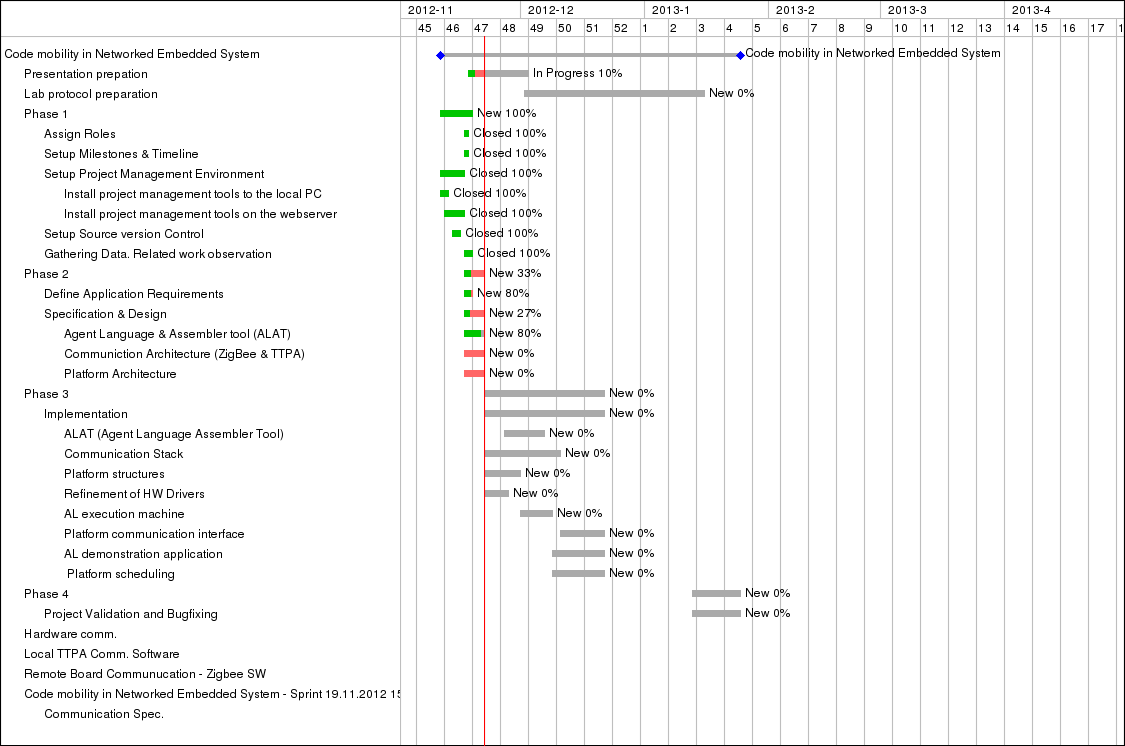
\includegraphics[scale=0.4]{figures/gantt.png}
\caption{Gantt Diagram of the Project}
\label{fig:ganttdiag}
\end{figure}


\begin{comment}
Interpreter for agent language:
\begin{itemize}
\item Agent language lexical analysis
\item Interpreter for agent language
%\item Agent language semantic analysis
\end{itemize}


Compiler for agent language:
\begin{itemize}
\item Agent language lexical analysis
\item Agent language syntax analysis
\item Agent language semantic analysis
\end{itemize}
}

Platform for mobile agents:

\begin{itemize}
\item Agent structure representation
\item Implementation of Agent structure
\item Implementation of Agent functions
\item Implementation of drivers
\item Implementation of scheduler
\item Implementation of communication protocols

\end{itemize}


%\chapter{Appendix 1}
%\chapter{Appendix 2}

%	\section{Standards}
%	\section{Training}
\end{comment}
% add other chapters and sections to suit

	\bibliography{protocol}

	\bibliographystyle{plain}

\end{document}

